\documentclass{article}
\usepackage{epsfig}
\usepackage{hyperref}
\usepackage[margin=1in]{geometry}

\renewcommand{\refname}{\centerline{References cited}}
\usepackage[numbers]{natbib}
\usepackage{graphicx}

\begin{document}
\pagestyle{empty}
\begin{center}
{\Large{\bf Intermediate Report}}\\*[3mm]
{\bf Mormon Heritage} \\*[3mm]

Christopher Mertin
\end{center}

The hardest part of the project has been completed. The parts that have been done have been the affine transformation and the facial averaging. The affine transformations were required to map the faces from the domain that they were in into the same domain as the other faces. To preserve facial features such as facial length, the mapping was done on the outside of the eyes such that the end points of each eye were at the same point. The image size was also standardized.

From here, an average of the face can be made. This average was made to be a ``ground truth'' between the two sets of photos, those with mormon heritage and those without. The averages can be used to try and see what features might be good in the clustering algorithm to reduce dimensionality. The figure below is an average of women confirmed to have mormon heritage.

\begin{figure}[!h]
\centering
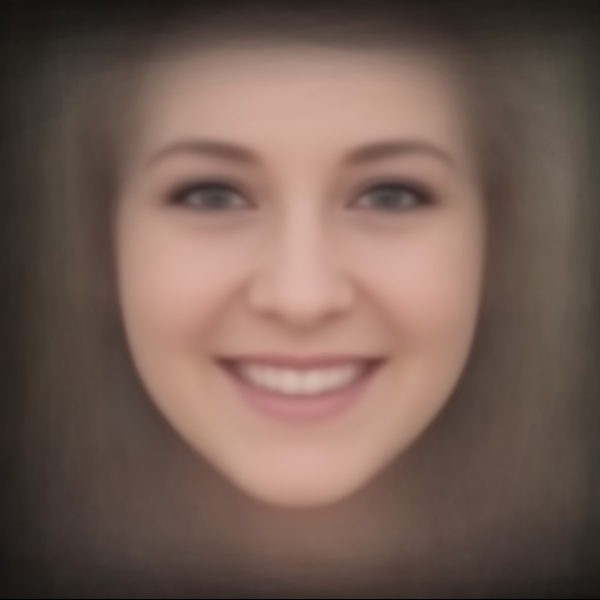
\includegraphics[width=.5\linewidth]{data/Provo_avg.jpg}
\end{figure}

There are slight differences in this photo and the averaged photo of those without mormon heritage, and we can point out these facial features to use those points for the clustering algorithm.

Now that the affine transformations are complete, the clustering algorithm with SIFT features can be used to see if there is some structure in the data. Along side this, the Eigenfaces algorithm can also be implemented quite easily, as it's simple linear algebra based on the images. All the data is collected, so all that needs to be done is translate the images to greyscale for the clustering and SVD algorithms. Code is already written to extract the SIFT features from the images, which was required to do the affine transformation. 

For the clustering algorithms, various clustering techniques will be looked at, along with the clustering size, to try and determine structure. With the topic of Eigenfaces, we can use PCA to attempt to determine how ``similar'' someone is to a group with or without Mormon heritage. It will be important to subtract the average (as seen in the above figure) from each of the sets as we want to find strucutre which might be hidden by the ``average face.''

\end{document}
